\newpage
\section{Durchführung}
\label{sec:Durchfuehrung}

\subsection{Die Feder}
\label{sec:feder}
Verwendet wird eine Trompetenfeder, welche in der Möbelbeschlagindustrie in Schubladeneinzugsystemen
verwendet wird. 
Der Federtyp zeichnet sich durch die nicht klassische Ösenform aus, welche die Problematik des Ösenbruchs umgeht.\\

Wichtig ist anzumerken, dass die Ruhelänge $L_0$ in der Praxis legiglich als anzustreben gilt.
Die Länge der Zugfeder vergrößert bei Belastung, deshalb bedarf es keiner festgeschrieben Maximallänge für $L_0$, da
der Einbauraum stehts auf eine großerwerdene Feder ausgelegt ist.  

\begin{center}
    \makebox[\textwidth]{
        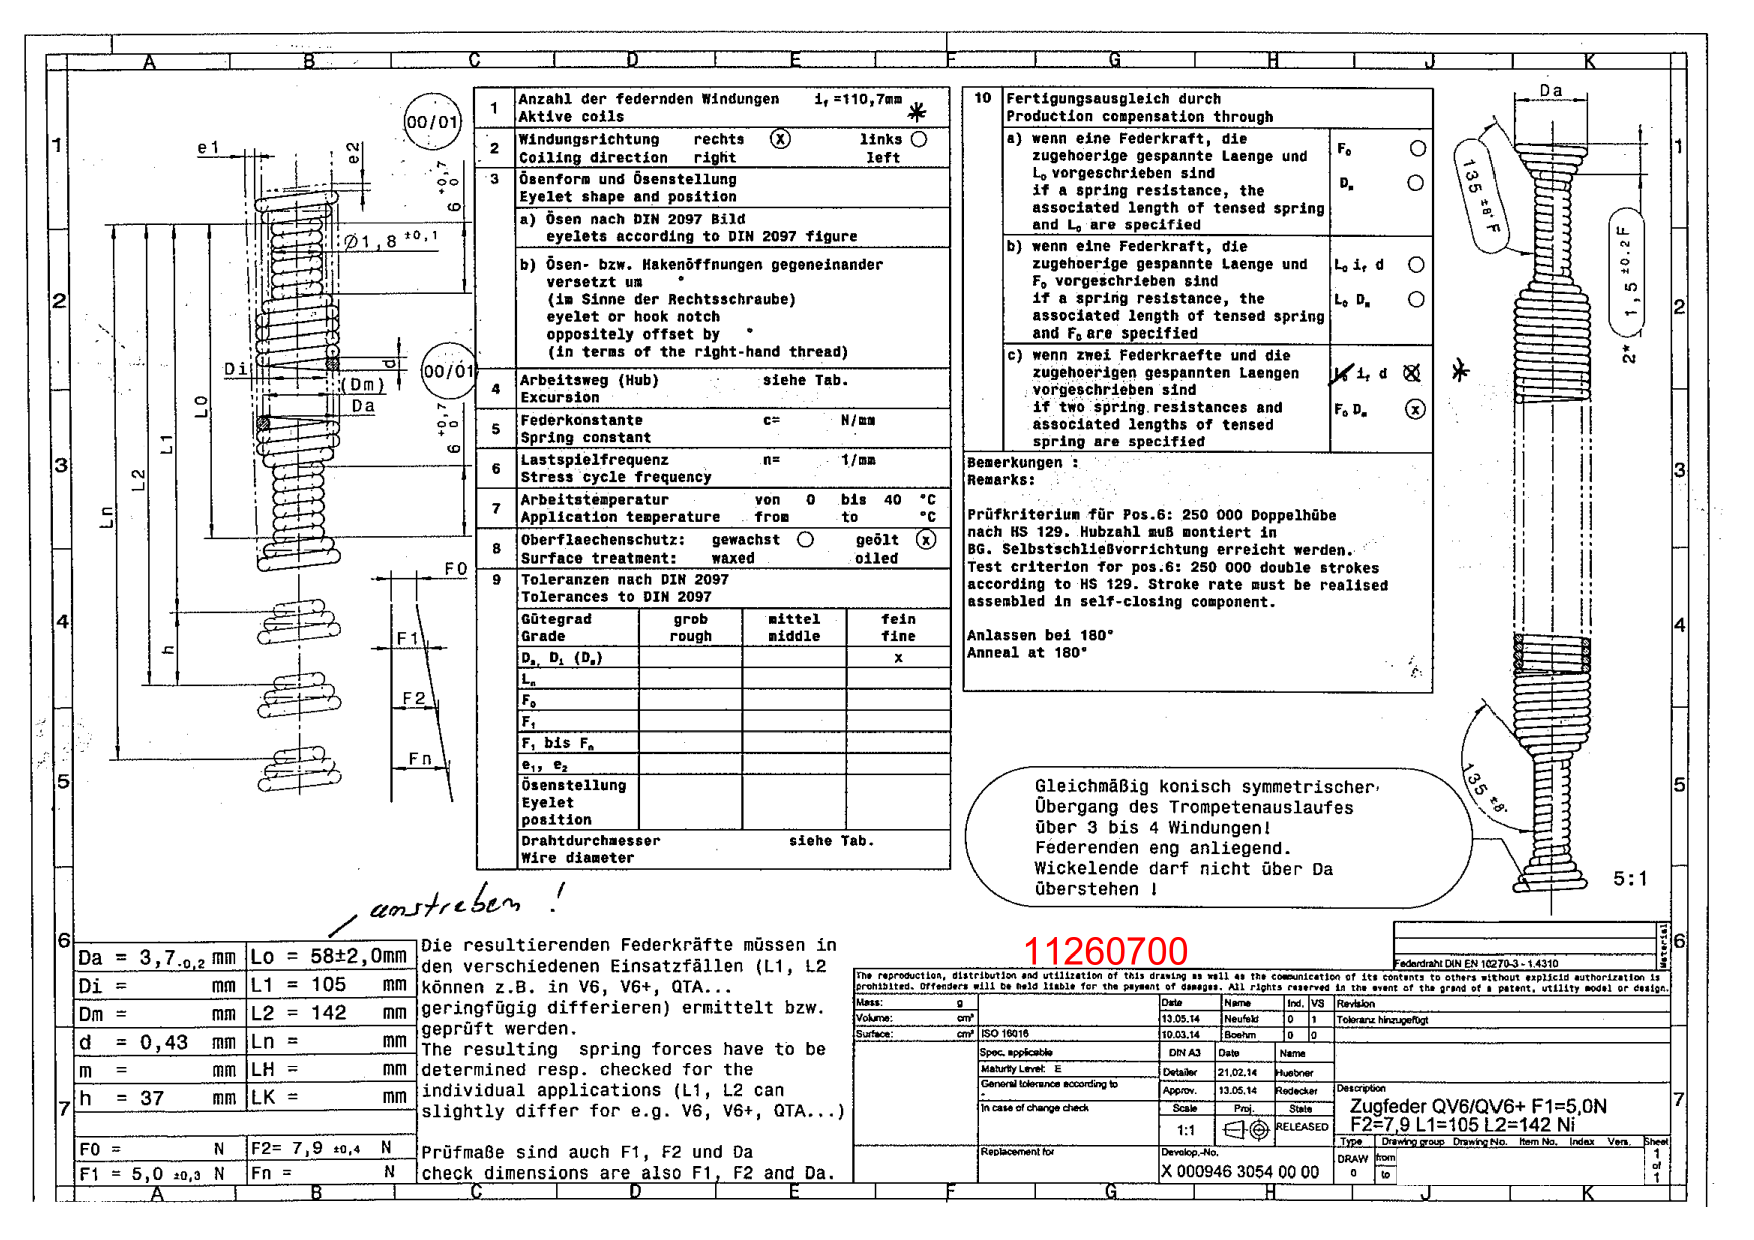
\includegraphics[width=\paperwidth]{bilder/zeichnung_11260700.pdf}
        \label{fig:zeichnung}
        }
\end{center}
Die Zeichnung zeigt die Feder mit einem Ausdurchmesser $D_a$ von $3,7\;\text{mm}$, diese Feder wird
als Basisfeder verwendet.\\ 

Im Folgenden kann die Feder als zylindrische Feder betrachtet werden,
da die Belastung in der Größenordung liegt, sodass der zu federnde Anteil nicht 
vom Trompentenanteil (gemeint sind hier die Ösenteile am Ende der Feder)
ausgeführt wird, da bei der Kraftprüfung die größte zulässige Prüflänge $Ln$ mit 
$Ln>L2$ nicht überschritten wird.

\subsection{Vorgehen}
Folgendes wird untersucht:
\begin{enumerate}
    \item   Die Basisfeder wird in einer Stückzahl von 6 anhand der Zeichnung produziert.\\
            Gemessen wird jeweils der Federaußendurchmesser $D_a$ und die Federlänge 
            $L0$ und die Gesamtmasse $m$ der 6 Federn sowie die Kräfte $F1$ und $F2$ an $L1$ und $L2$ mithilfe eines Newtonkraftmesser\ref{fig:kraftmesser}.
            Dort können die Federn gespannt werden und auf die zuprüfenden Längen gestreckt werden.\\
            Anschließend werden die Werte $D_a$, $L0$, $F1$ und $F2$ gemittelt (Feder 1).

    \item   Nun wird der Federaußendruchmesser $D_a$ um ca. $\pm1$mm varriert und in einer 
            Stückzahl von jeweils 5 produziert.\\
            Die Federn werden an $D_a$, $L0$, $m$, $F1$ und $F2$ vermessen und gemittelt (Feder 2, Feder 3).\\
            Die gemittelte Federn (Feder 1,2,3) werden in einem Kraft-Weg-Diagramm eingetragen und
            die Federraten $R$ über die Steigung einer Ausgleichsgeraden, sowie die Vorspannkraft $F0$ 
            über den y-Achsenabschnitt bestimmt.\\
            Anschließend wird der Einfluss der Federdicke $D$ auf die Federkonstante $R$ ermittelt
            und nach Gl. \ref{eqn:federrate} $R \propto D^{-3}$ gefittet und mit der Theoriekurve verglichen.

    \item   Nun wird die Windungszahl $n$ um ca. $\pm 10$ Windungen varriert und in einer Stükzahl von 5 produziert.(Feder 4, Feder 5)\\
            Es wird analog zu 2 vermessen und gemittelt und ein Kraft-Weg-Diagramm erstellt und
            daraus $R$ und $F0$ aus einer Ausgleichgeraden ermittelt und mit der Theoriekurve verglichen.
            Anschließend wird der Einfluss der wirkenden Wicklungszahl $n_{wirk}$ auf die Federkonstante $R$ ermittelt
            und nach Gl. \ref{eqn:federrate} $R \propto n_{wirk}^{-1}$ gefittet und mit der Theoriekurve verglichen.

    \item   $R$ in abhängigkeit von $m$\\
            $m$ in abhängigkeit von $D$ und $n_{wirk}$  
\end{enumerate}
 